
%opening
\title{Animation der TableView}
\author{Burak Erol, Philipp Winterholler}

\section{Animation der TableView}

Um eine �bersicht aller gefundenen Sech Tags grafisch darzustellen, wurde ein Label ��ber den Sech-Button erg�nzt, welche die Anzahl der Sech-Tags in einer roten Schrift angibt. Diese Anzahl soll dem Nutzer zeigen, wie viele Sech Tags sich auf der Webseite befinden. Beim Bedienen des Sech Buttons, wird die Sech Tabelle animiert herbei gerufen. Diese Tabelle wird rechts im Browser ein- und ausgefahren. Das WKWebView wird dementsprechend vergr�ߟert oder verkleinert. Bedient man diesen Sech Button, so f�hrt sich eine Tabelle vom rechten Bildschirm aus und liefert alle Tags in einer TableView zur��ck. Die zur�ckgelieferten Tags werden in seperaten Zellen auf der TableView abgespeichert, die durch anklicken eine neue Pop-Up Seite, spezifisch zu dem angeklickten Tag, �ffnet. Aufgrund der Umstellung der Navigationsleiste wird diese grafische Darstellung der Anzahl an Sech-Tags nicht mehr angezeigt. Die Umstellung der Navigationsleiste war notwendig um die H�he und Breite des WKWebViews festzulegen, darum ist ein neuer Navigation Controller erzeugt worden, welche die Navigation Bar automatisch mitliefert. In die neue Navigation Bar kann jedoch kein Label hinzugef�gt und spezifisch positioniert werden, somit wurde diese Option entfernt. 


\includegraphics[width=12cm]{Pics/Sech_Anzahl}
\newpage
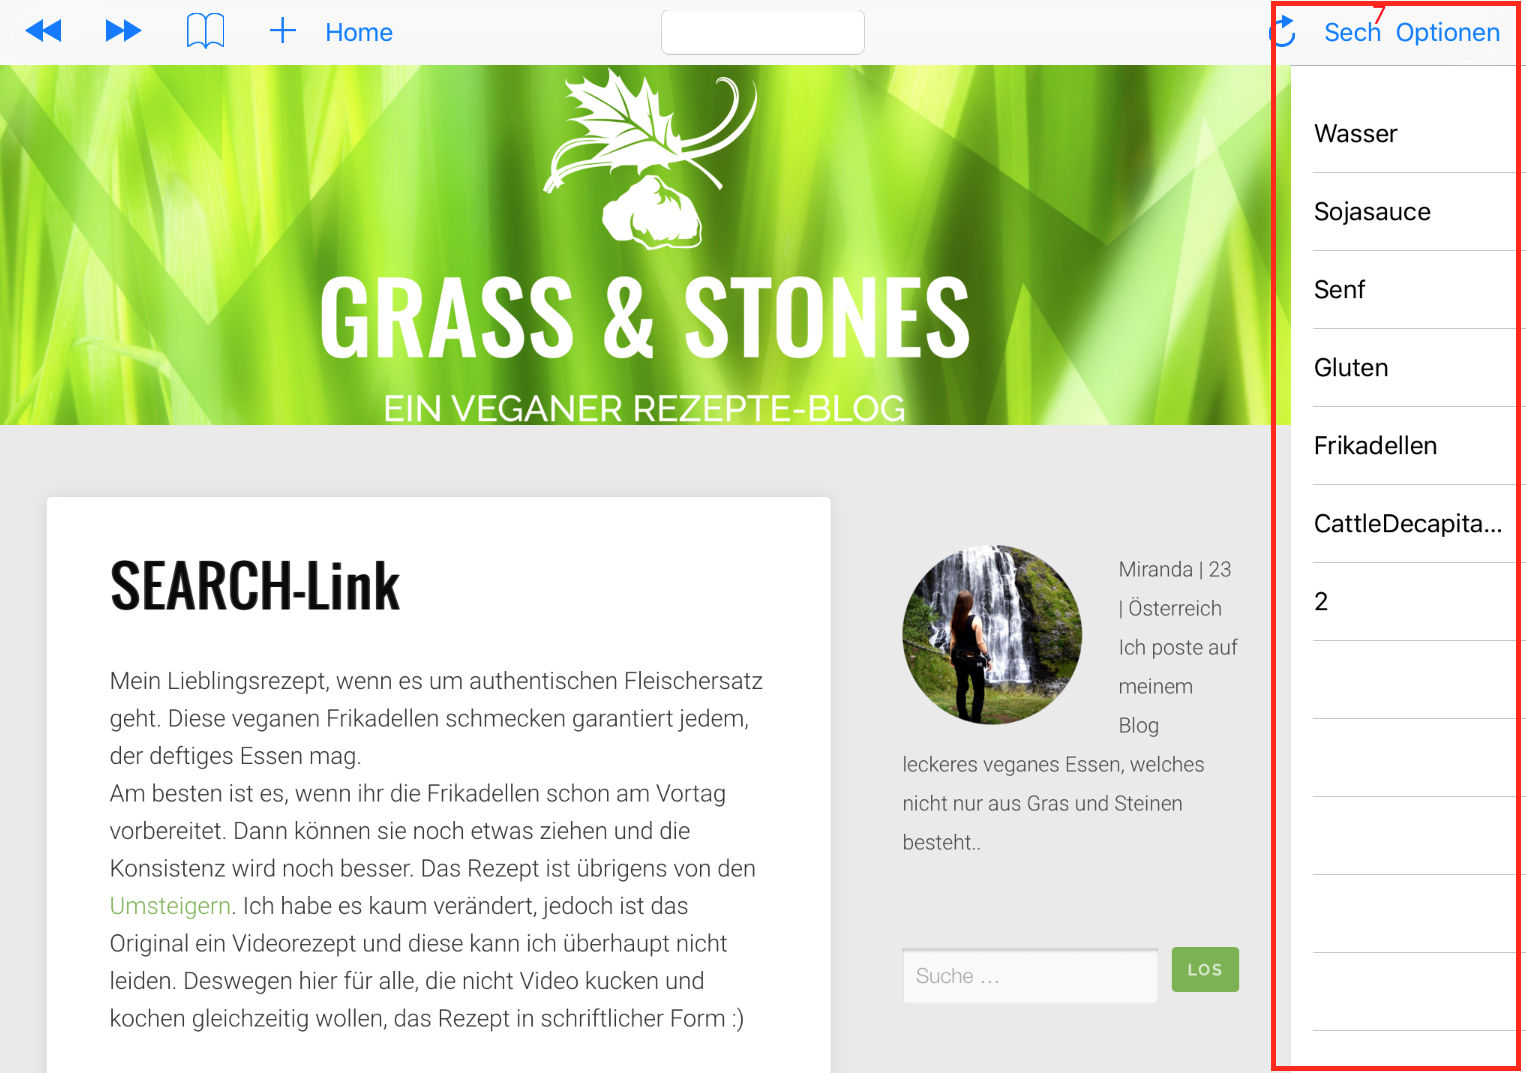
\includegraphics[width=12cm]{Pics/Sech_Tabelle_aufgeklappt}
\newpage

\includegraphics[width=12cm]{Pics/Sech_Tabelle_versteckt}


